\chapter{aCoral启动}
2440上电之后,CPU将从0地址处开始取指执行指令。如果将aCoral程序存放在Norflash中,并通过mini2440开关S2选择Norflash启动,则Norflash从硬件层面上被映射为0地址开始的一段地址;
如果将aCoral放在Nandflash中,并且通过S2开关选择Nandflash启动,则开发板在上电后自动将Nandflash前4KB内容复制到开发板上的一块SRAM中。
这块SRAM我们称为Stepping Stone(垫脚石),并且Stepping Stone的地址就是从0地址开始。所以,不论选择何种启动方式,2440都将从0地址开始执行第一行代码。

图\ref{复位后S3C2440A的存储器映射}显示了复位后S3C2440A的存储器映射情况,详细请参考《S3C2440中文手册》第五章。
\begin{figure}[H]
	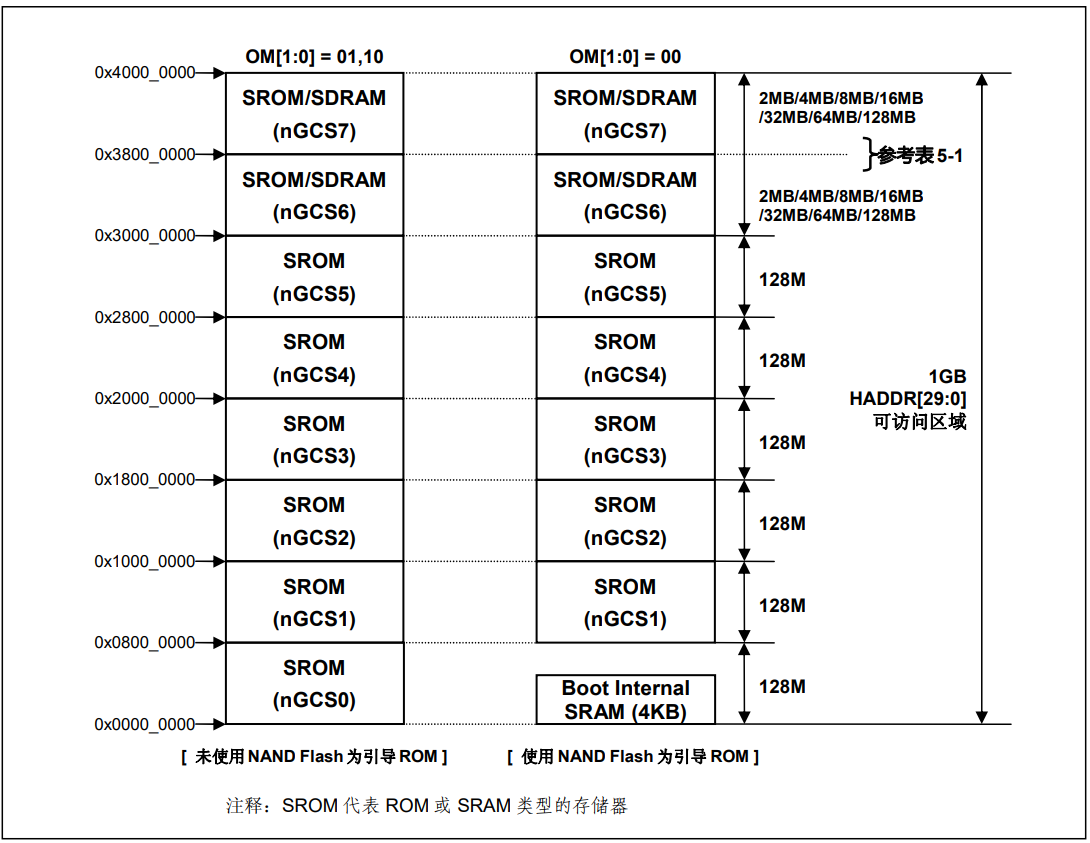
\includegraphics[width=\textwidth]{复位后S3C2440A的存储器映射.png}
	\caption{复位后S3C2440A的存储器映射}
	\label{复位后S3C2440A的存储器映射}
\end{figure}

\section{启动-第一阶段}
之前说到,aCoral的bootloader其实就是
\begin{lstlisting}
 hal/s3c2440/src/start.S 
\end{lstlisting}

我们将其称为aCoral的启动文件。启动文件中,这行跳转指令就是整个aCoral的入口,将被烧录在Nandflash或Norflash的0地址。
\begin{lstlisting}
__ENTRY:
	b	ResetHandler
\end{lstlisting}

这句跳转程序将跳转到ResetHandler标号处,执行一些上电之后的硬件初始化工作,包括关闭看门狗、配置时钟、堆栈初始化、复制OS到SDRAM等。
我们一点点来看这些代码。

PS:请准备好《S3C2440中文手册》

\subsection{禁用看门狗}
\begin{lstlisting}
	@ disable watch dog timer
	mov r1, #0x53000000
	mov	r2, #0x0
	str	r2, [r1]
\end{lstlisting}

看门狗WatchDog的名字形象的描述了它的工作原理,看门狗每隔一段时间(比如:3个小时)它就会饥饿,每次饥饿时都叫,如果不想让它叫,只要我们保证在3个小时内喂狗一次就行。因此我们要及时的对看门狗控制器执行喂狗操作。
看门狗定时器内部有一个递减计数器,当该计数器递减为0的时候,就会自动重启控制器,如果我们写有这样的程序,该程序在定时器计数器递减为0之前,将其递减计数器重新设置一下(喂狗),那么就不会产生重启操作。假如机器设备出现异常情况下如死机,CPU执行出错,程序跑飞等情况,CPU就会陷入非正常的执行流程,就不会去执行重置计数器的程序,当计数器递减为0时,会产生复位控制器信号,机器就会重新启动,恢复正常执行流程。这样的设计原理就解决了很多环境恶劣的情况下,对服务器进行重启的任务。上面的重置倒计数的操作通常叫做“喂狗”。
为了避免看门狗带来的影响,简化系统,我们选择关闭看门狗。

上述代码向地址0x53000000(r1),也就是看门狗定时器控制寄存器(WTCON)写入了0x0000(r2),即16个0。
结合图\ref{看门狗},可以知道,这样配置的结果就是禁止了看门狗,系统也就不需要定时去喂狗了。

当然了,在比较正式的系统中,看门狗是必须要开启的,防止系统一直死机。这里由于我们只是在开发aCoral,所以暂时关闭。


\begin{figure}[H]
	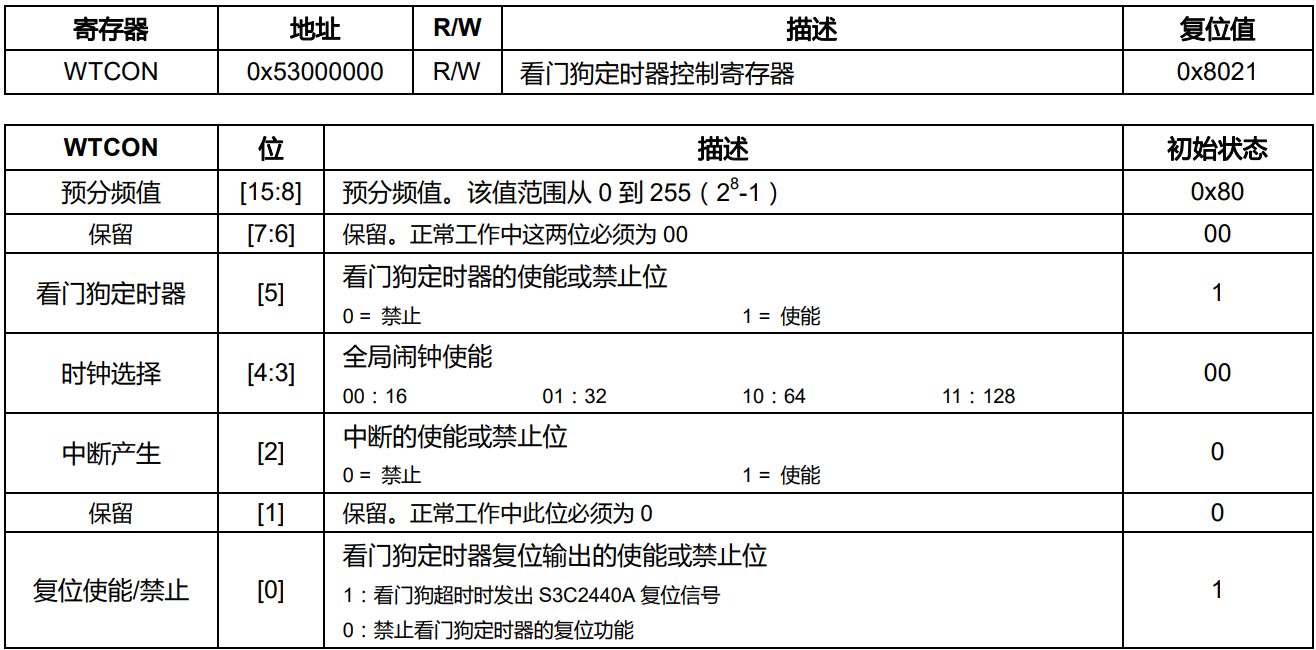
\includegraphics[width=\textwidth]{看门狗.png}
	\caption{看门狗定时器控制(WTCON)寄存器(手册第18章)}
	\label{看门狗}
\end{figure}
\subsection{关中断}
\begin{lstlisting}
	@ disable all interrupts
	mov	r1, #INT_CTL_BASE
	mov	r2, #0xffffffff
	str	r2, [r1, #oINTMSK]
	ldr	r2, =0x7ff
	str	r2, [r1, #oINTSUBMSK]
\end{lstlisting}

系统刚上电启动,这个时候,aCoral的中断系统还没有初始化,此时发生中断我们无法处理,所以要关闭中断。

代码中,立即数 INT\_CTL\_BASE = 0x4A000000 ,立即数 oINTMSK = 0x08 ,两个立即数相加的地址即指向中断屏蔽寄存器。中断屏蔽寄存器由 32 位组成,其每一位都都涉及一个中断源。如果某个指定为被设置为 1,则 CPU 不会去服务来自
相应中断源(请注意即使在这种情况中,SRCPND 寄存器的相应位也设置为 1)的中断请求。如果屏蔽位为 0,则
可以服务中断请求,如图\ref{中断屏蔽寄存器}。

oINTSUBMSK指向的次级中断屏蔽寄存器类似。

\begin{figure}[H]
	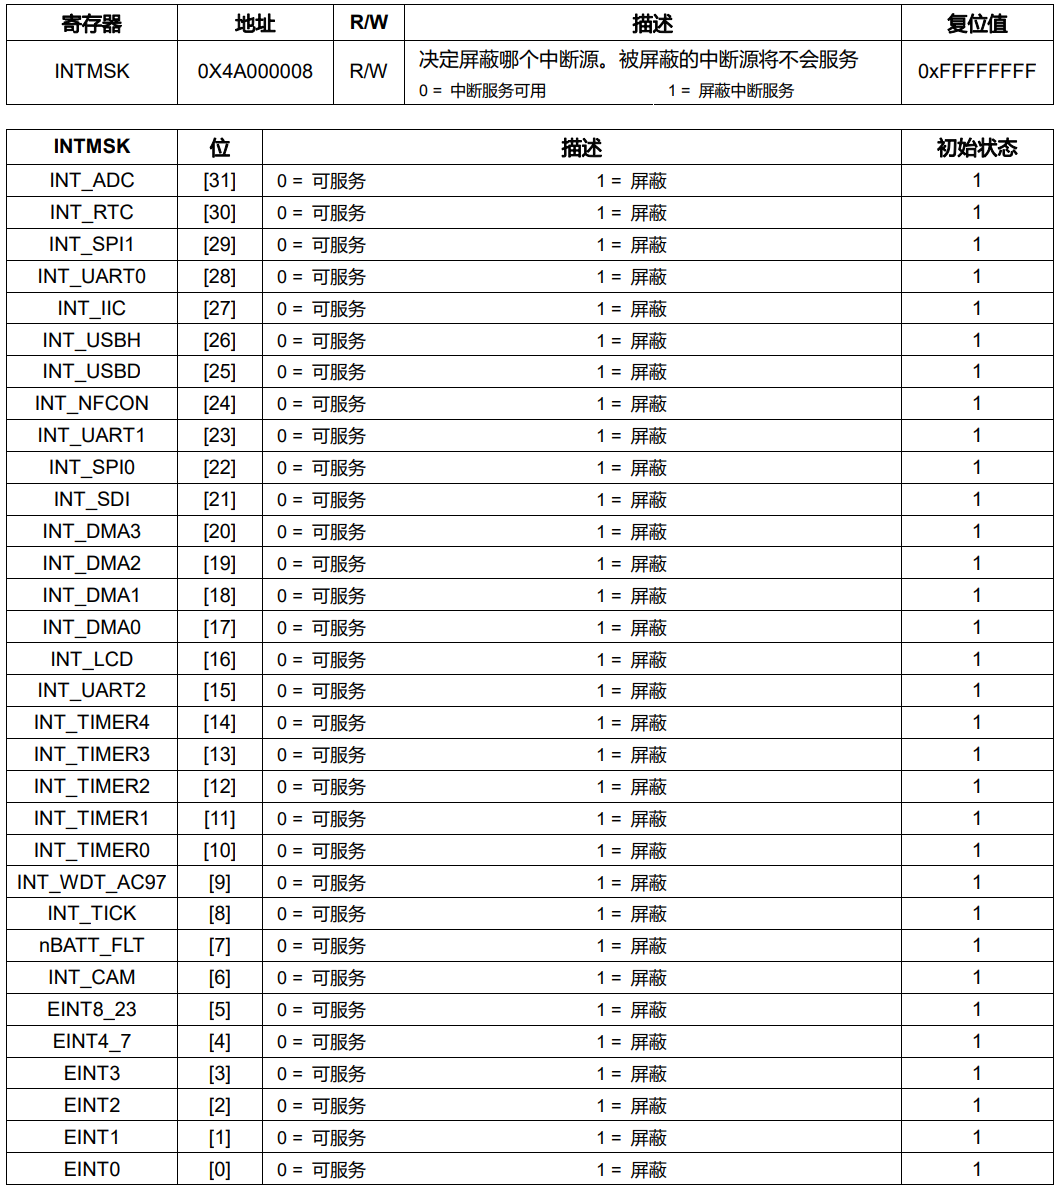
\includegraphics[width=\textwidth]{中断屏蔽寄存器.png}
	\caption{中断屏蔽寄存器(手册第14章)}
	\label{中断屏蔽寄存器}
\end{figure}


\section{时钟初始化}
\begin{lstlisting}
	@ initialise system clocks
	mov	r1, #CLK_CTL_BASE
	mvn	r2, #0xff000000
	str	r2, [r1, #oLOCKTIME]

	mov	r1, #oCLKDIVN
	mov	r2, #M_DIVN
	str	r2, [r1, #oCLKDIVN]

	mrc	p15, 0, r1, c1, c0, 0	@ read ctrl register
	orr	r1, r1, #0xc0000000	@ Asynchronous
	mcr	p15, 0, r1, c1, c0, 0	@ write ctrl register

	mov	r1, #CLK_CTL_BASE
	ldr 	r2, =vMPLLCON	        @ clock user set
	str	r2, [r1, #oMPLLCON]
\end{lstlisting}

mini2440上电后,系统工作在板载晶振12MHz的频率下。这个频率比较低,系统的性能还没有完全得到发挥,所以需要激发一下潜能,使用一种叫做锁相环PLL的东西来倍频,加倍之后的频率再给CPU和板子上的其他设备使用。

mini2440有两个锁相环,MPLL和UPLL。
MPLL的输出频率直接给CPU使用,称为FCLK,同时经过上面初始化系统时钟后得到另外两个频率HCLK和PCLK,分别给板载高速硬件和低速外设使用。

将 M\_DIVN = 0x5 写入 oCLKDIVN + oCLKDIVN = 0x4C000014 寄存器后,三者的比例为FCLK:HCLK:PCLK=8:2:1,如图\ref{时钟分频控制寄存器}
\begin{figure}[H]
	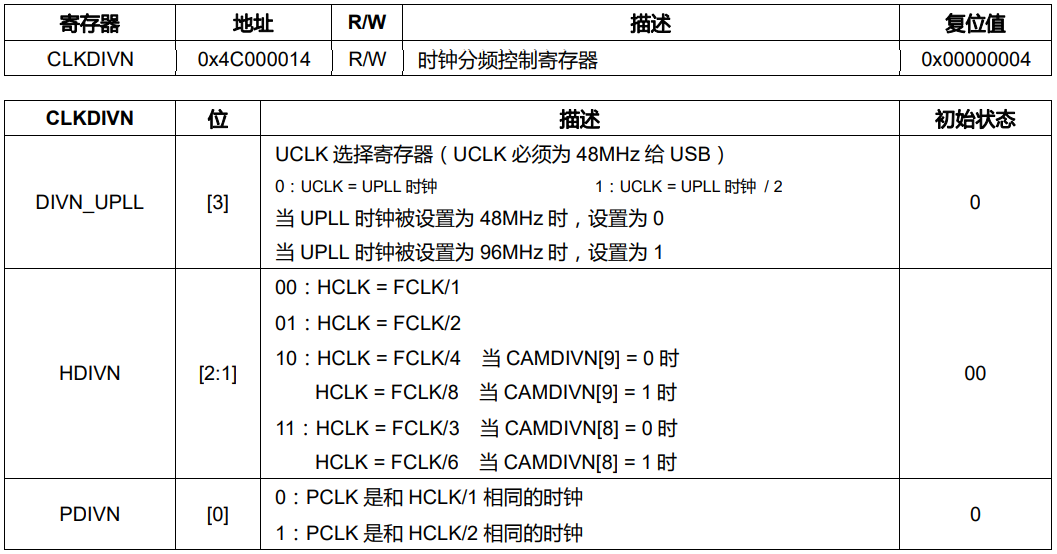
\includegraphics[width=\textwidth]{时钟分频控制寄存器.png}
	\caption{时钟分频控制寄存器(手册第7章)}
	\label{时钟分频控制寄存器}
\end{figure}

将 vMPLLCON = 0x1FC0021 写入 oMPLLCON + CLK\_CTL\_BASE = 0x4C000004 寄存器后,得到FCLK≈400MHz,再根据之前的比例得到HCLK 和 PCLK分别为100MHz和50MHz。
计算过程见图\ref{PLL 控制寄存器},其中Fin就是晶振的频率=12MHz。
\begin{figure}[H]
	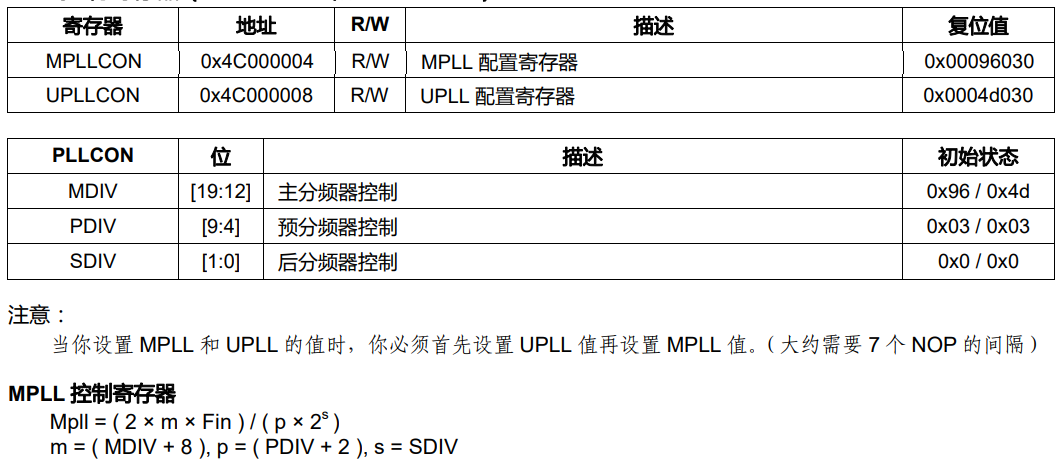
\includegraphics[width=\textwidth]{PLL 控制寄存器.png}
	\caption{PLL 控制寄存器(手册第7章)}
	\label{PLL 控制寄存器}
\end{figure}

UPLL的输出频率没有配置,直接给USB使用。


\subsection{存储空间初始化}
\begin{lstlisting}
	bl	memsetup
......
	@*************************************
	@ initialise the static memory
	@ set memory control registers
	@*************************************
memsetup:
	mov	r1, #MEM_CTL_BASE
	adrl	r2, mem_cfg_val
	add	r3, r1, #52
1:	ldr	r4, [r2], #4
	str	r4, [r1], #4
	cmp	r1, r3
	bne	1b
	mov	pc, lr
\end{lstlisting}

memsetup就是初始化一下mini2440的存储器(BANK0~BANK7),具体自行阅读《S3C2440中文手册》第5章。

\subsection{栈初始化}
\begin{lstlisting}
	bl      InitStacks
......
	@************************************
	@             堆栈初始化
	@************************************

InitStacks:
	mov r2,lr
	mrs	r0,cpsr
	bic	r0,r0,#MODE_MASK
	orr	r1,r0,#UND_MODE|NOINT
	msr	cpsr_cxsf,r1		@UndefMode
	ldr	sp,=UDF_stack		@ UndefStack=0x33FF_5C00

	orr	r1,r0,#ABT_MODE|NOINT
	msr	cpsr_cxsf,r1		@AbortMode
	ldr	sp,=ABT_stack		@ AbortStack=0x33FF_6000

	orr	r1,r0,#IRQ_MODE|NOINT
	msr	cpsr_cxsf,r1		@IRQMode
	ldr	sp,=IRQ_stack		@ IRQStack=0x33FF_7000

	orr	r1,r0,#FIQ_MODE|NOINT
	msr	cpsr_cxsf,r1		@FIQMode
	ldr	sp,=FIQ_stack		@ FIQStack=0x33FF_8000

	bic	r0,r0,#MODE_MASK|NOINT
	orr	r1,r0,#SVC_MODE
	msr	cpsr_cxsf,r1		@SVCMode
	ldr	sp,=SVC_stack		@ SVCStack=0x33FF_5800

	mrs     r0,cpsr
	bic     r0,r0,#MODE_MASK
	orr     r1,r0,#SYS_MODE|NOINT
	msr     cpsr_cxsf,r1    	@ userMode
	ldr     sp,=SYS_stack

	mov	pc,r2
\end{lstlisting}

InitStacks就是初始化一下arm处理器各个模式的栈。因为影子寄存器的存在,每个模式的sp寄存器都是独立的(除了系统和用户模式)。
具体的做法就是通过修改cpsr寄存器的[5:0]位,进入每一个模式并修改sp寄存器位该模式的栈底地址。
每个模式的栈底地址定义于链接脚本。链接脚本将在下一节进行讲解。cpsr寄存器各位编排如图\ref{程序状态寄存器格式}。
\begin{figure}[H]
	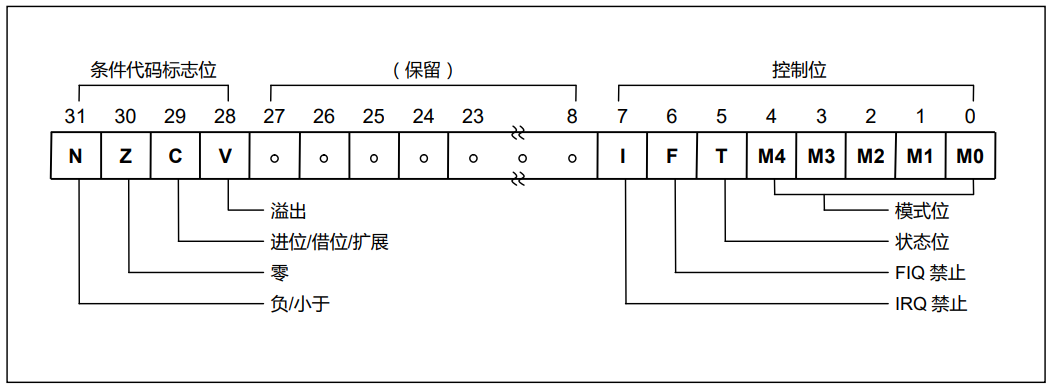
\includegraphics[width=\textwidth]{程序状态寄存器格式.png}
	\caption{程序状态寄存器格式(手册第2章)}
	\label{程序状态寄存器格式}
\end{figure}

PS:关于影子寄存器(也称分组寄存器),请查看《S3C2440中文手册》第2章图2-3。


\subsection{自我拷贝(loader)}
\begin{lstlisting}
	adr  r0,__ENTRY
	ldr  r1,_text_start
	cmp  r0,r1
	blne copy_self  
...
copy_self:

	ldr	r1, =( (4<<28)|(2<<4)|(3<<2) )	/* address of Internal SRAM  0x4000002C*/
	mov	r0, #0		
	str	r0, [r1]


	mov	r1, #0x2c	/* address of men  0x0000002C*/
	ldr	r0, [r1]
	cmp	r0, #0
	bne	copy_from_rom
        
    ldr	r0, =(2440)
	ldr	r1, =( (4<<28)|(2<<4)|(3<<2) )
	str	r0, [r1]
	b       copy_from_nand 
\end{lstlisting}

这一步非常重要。如果aCoral是烧写在nor flash中,启动时是从0地址开始运行的,那aCoral怎么到内存SDRAM(起始地址为0x30000000)中运行呢?
这项任务是由aCoral自己来完成的,也就是我搬起了我自己。可以看到copy\_self的执行条件

\subsection{bss段清零}
\begin{lstlisting}
	ldr  r0,_bss_start
	ldr  r1,_bss_end
	bl    mem_clear
.......
	@***********************************
	@ clear memory
	@ r0: start address
	@ r1: length
	@***********************************

mem_clear:
	mov r2,#0
1:	str r2,[r0],#4
	cmp r0,r1
	blt 1b
	mov pc,lr
\end{lstlisting}

bss段中的数据都是未初始化或者初始值为0的,所以清空bss段就是将其中的内存全部赋值为0。
mem\_clear的两个参数分别为bss段的起始地址和结束地址,都定义在链接脚本中。

\subsection{跳转至下一阶段}
\begin{lstlisting}
	ldr    pc,=acoral_start	
\end{lstlisting}

代码最终将寄存器pc设置为acoral\_start的值,表示CPU将跳转到acoral\_start函数处执行。acoral\_start函数位于
\begin{lstlisting}
 kernel\include\core.c
\end{lstlisting}
\section{启动-第二阶段}

core.c中的acoral\_start()函数如下

这部分代码中,最重要的就是acoral\_module\_init()这个函数。这个函数将初始化aCoral的各个模块,包括中断、内存、线程等嵌入式操作系统必需的模块。初始化完成后,执行acoral\_core\_cpu\_start()函数,aCoral开始运行。

